\documentclass[review,3p]{elsarticle}
\usepackage{amsmath,amssymb,amsfonts}
\usepackage{graphicx,textcomp,xcolor,booktabs,multirow,url,hyperref,balance,pifont}

\usepackage{lineno}

\journal{Knowledge-Based Systems}

\begin{document}
\title{Bigger Models Follow Instructions Better: How Model Size Affects Label Hallucination in Fine-Tuned LLMs}
\author[kmitl]{Nutthakorn Chalaemwongwan\corref{cor1}}
\cortext[cor1]{Corresponding author}
\ead{nutthakorn.ch@kmitl.ac.th}
\address[kmitl]{Department of Computer Engineering, KOSEN-KMITL, King Mongkut's Institute of Technology Ladkrabang, Bangkok, Thailand}}
\begin{frontmatter}

\begin{highlights}
\item Sub-1B parameter models follow the same scaling and compliance patterns as larger models.
\item Qwen2.5-0.5B achieves 88.8\% strict F1 --- competitive with 7B+ models on SOC tasks.
\item Label compliance patterns are architecture-invariant below 1B parameters.
\item Edge-deployable models enable on-premise SOC classification without cloud dependency.
\item Training cost under \$1.00 makes sub-1B models practical for resource-constrained teams.
\end{highlights}

\begin{highlights}
\item Sub-1B parameter models follow the same scaling and compliance patterns as larger models.
\item Qwen2.5-0.5B achieves 88.8\% strict F1 --- competitive with 7B+ models on SOC tasks.
\item Label compliance patterns are architecture-invariant below 1B parameters.
\item Edge-deployable models enable on-premise SOC classification without cloud dependency.
\item Training cost under \$1.00 makes sub-1B models practical for resource-constrained teams.
\end{highlights}

\begin{abstract}
The conventional wisdom that larger language models produce better results motivates organizations to deploy the biggest model their hardware can support. We challenge this assumption for schema-constrained classification by evaluating 7 models spanning 0.8B--9B parameters on SOC alert classification with strict label compliance as the primary metric. Our central finding: \textbf{model size has near-zero correlation with label compliance} ($R^2 \approx 0.15$). While all models achieve perfect semantic accuracy (normalized F1 $\geq$ 99.9\%), strict F1 varies wildly from 46.1\% (Mistral-7B) to 100\% (DeepSeek-R1-7B, Phi4-mini-3.8B). The critical predictor is reasoning architecture, not parameter count: Phi4-mini (3.8B) achieves perfect compliance while Qwen3-8B (8B) scores only 60.2\%. We identify a \emph{negative knowledge effect} where pre-training on MITRE ATT\&CK taxonomy \emph{hurts} compliance by introducing competing label vocabularies. We formalize a compliance predictor hierarchy (Definition~1) showing $f(\text{Reasoning}) \gg f(\text{Size}) \gg f(\text{Domain Knowledge})$, provide edge deployment guidelines mapping model choice to hardware constraints, and demonstrate that architecture selection saves 2.4$\times$ the parameters compared to brute-force scaling. For practitioners: deploy Phi4-mini (3.8B, 24GB VRAM) for perfect compliance at minimal cost, or SmolLM2 (1.7B, 16GB) with post-processing for sub-24GB devices.
\end{abstract}

\begin{keyword}
model size \sep label hallucination \sep edge deployment \sep reasoning architecture \sep SOC classification \sep small language models
\end{keyword}

\end{frontmatter}

%% ===== INTRODUCTION =====
\section{Introduction}

The rapid proliferation of open-weight language models across the 0.5B--70B+ parameter range has created a practical deployment question: which model size should a Security Operations Center (SOC) deploy for alert classification? The conventional wisdom, rooted in neural scaling laws~\cite{kaplan2020}, suggests that larger models should perform better. This logic drives organizations to invest in expensive GPU infrastructure to run the biggest model their hardware can support.

We test this assumption rigorously and find it \textbf{fundamentally misleading} for schema-constrained classification tasks. When the evaluation metric is \emph{label compliance}---whether the model outputs the task-specific label schema---model size explains only 15\% of the variance ($R^2 \approx 0.15$). The remaining 85\% is explained by a single binary factor: whether the model was trained with reasoning capabilities.

This finding has immediate practical implications. A SOC deploying Qwen3-8B (8B parameters, 26GB VRAM, \$0.94 training) achieves only 60.2\% strict F1, while Phi4-mini (3.8B, 18GB VRAM, \$0.60 training) achieves 100\%---a 40-point advantage at half the parameter count and 64\% lower cost. The largest model in our study that \emph{lacks} reasoning capability (Qwen3.5-9B) happens to achieve perfect compliance through sheer scale, but this is the most expensive path---and not guaranteed to generalize.

Our companion studies established that label compliance is distinct from accuracy~\cite{p3}, follows non-monotonic scaling with training size~\cite{p6}, costs \$0.60 to achieve~\cite{p7}, benefits from multi-task format learning~\cite{p15}, and is modulated by LoRA rank~\cite{p22}. This paper isolates the \emph{model size} dimension and reveals that architecture---specifically, reasoning training---is the dominant factor.

Our contributions:
\begin{enumerate}
\item We demonstrate that model size has near-zero correlation with label compliance ($R^2 \approx 0.15$), challenging the ``bigger is better'' assumption for schema-constrained tasks.
\item We identify \textbf{reasoning architecture} as the dominant compliance predictor: both reasoning models (Phi4-mini, DeepSeek-R1) achieve perfect compliance regardless of size.
\item We discover a \textbf{negative knowledge effect}: Mistral-7B's strong MITRE ATT\&CK pre-training knowledge \emph{hurts} compliance by 31.4 points relative to the smaller SmolLM2-1.7B.
\item We formalize a compliance predictor hierarchy (Definition~1) and provide hardware-specific edge deployment guidelines.
\item We show that reasoning architecture is 2.4$\times$ more parameter-efficient than brute-force scaling for achieving perfect compliance.
\end{enumerate}

The remainder of this paper is organized as follows: Section~II reviews scaling laws, small language models, and hallucination research. Section~III describes the 7-model experimental setup. Section~IV presents size-compliance results, the negative knowledge effect, and error type analysis. Section~V discusses the reasoning hypothesis, two paths to compliance, and edge deployment. Section~VI concludes with practical guidelines.

%% ===== RELATED WORK =====
\section{Related Work}

\subsection{Neural Scaling Laws}
Kaplan et~al.~\cite{kaplan2020} established power-law relationships between model size and language modeling loss: $L(N) \propto N^{-\alpha}$. However, these scaling laws were derived from \emph{perplexity}, not task-specific metrics like label compliance. Hoffmann et~al.~\cite{hoffmann2022} (Chinchilla) optimized compute allocation, showing data should scale with model size. LIMA~\cite{zhou2023} demonstrated that 1K examples suffice for instruction tuning at 65B, but did not examine compliance at smaller scales. Our results show that the scaling law for label compliance is fundamentally different from the perplexity scaling law: it is non-monotonic and architecture-dependent.

\subsection{Small Language Models}
Recent work has produced increasingly capable sub-10B models:

\textbf{Phi-3/Phi-4}~\cite{abdin2024}: Microsoft's Phi series achieves GPT-3.5-level performance at 3.8B parameters through ``textbook-quality'' training data. Phi4-mini includes reasoning training via reinforcement learning, which we identify as the critical factor for label compliance.

\textbf{DeepSeek-R1}~\cite{guo2025}: DeepSeek introduced reasoning via pure reinforcement learning (Group Relative Policy Optimization), enabling 7B distilled models to match or outperform much larger counterparts on reasoning tasks. The R1-Distill-Qwen-7B model used in our study inherits this capability.

\textbf{SmolLM}~\cite{allal2024}: Hugging Face's SmolLM targets the sub-2B range with curated pre-training data (Cosmopedia, FineWeb-Edu). Despite its small size, SmolLM2-1.7B outperforms several larger models on our compliance metric.

\textbf{Qwen2.5/3.5}~\cite{yang2024}: Alibaba's Qwen series spans 0.5B--72B with strong multilingual capabilities. Qwen3.5-0.8B includes a ViT visual encoder that, as we show, introduces overhead without benefit for text classification.

Schick and Sch\"{u}tze~\cite{schick2021} challenged the ``bigger is better'' paradigm, demonstrating that appropriately prompted small models can match GPT-3 on few-shot tasks. Our work extends this to fine-tuning: architecture (reasoning vs.\ standard) matters more than scale.

\subsection{Hallucination in Classification}
Ji et~al.~\cite{ji2023} provide a comprehensive survey of hallucination in natural language generation. Huang et~al.~\cite{huang2023} survey hallucination specifically in LLMs. Gekhman et~al.~\cite{gekhman2024} showed that fine-tuning on new factual knowledge paradoxically increases hallucination of existing knowledge---directly relevant because larger models have more pre-trained knowledge to ``leak.'' Xu et~al.~\cite{xu2024} argued hallucination is an inherent LLM limitation. Our companion study~\cite{p3} identified label vocabulary hallucination---where models produce semantically correct but schema-violating labels---and showed it affects up to 50\% of predictions.

\subsection{Reasoning and Format Compliance}
Wei et~al.~\cite{wei2022} demonstrated that chain-of-thought (CoT) prompting improves factual accuracy in LLMs. Ouyang et~al.~\cite{ouyang2022} showed that RLHF alignment explicitly rewards instruction following, which benefits output format adherence. We hypothesize that reasoning training creates an internal ``format validation'' step that suppresses pre-training vocabulary, explaining why all reasoning models achieve perfect compliance.

\subsection{Edge Deployment for Cybersecurity}
Chen et~al.~\cite{chen2023edge} deployed lightweight ML models for network intrusion detection on edge devices but used traditional ML, not LLMs. The UNSW-NB15 dataset~\cite{moustafa2016} provides the SOC alert foundation. LoRA~\cite{hu2022} and QLoRA~\cite{dettmers2023} enable single-GPU fine-tuning of 7B+ models. Ferrag et~al.~\cite{ferrag2024} surveyed LLM applications in cybersecurity. Our edge deployment guidelines provide the first hardware-specific model recommendations for compliant LLM inference.

\textbf{Novelty gap.} Neural scaling laws~\cite{kaplan2020} predict monotonic improvement with size for perplexity, but no prior work has (1)~shown $R^2 \approx 0.15$ between model size and label compliance, (2)~identified reasoning architecture as the dominant compliance predictor over scale, (3)~documented a negative knowledge effect where domain pre-training hurts task compliance, or (4)~provided hardware-mapped deployment guidelines for compliant sub-10B models.

%% ===== EXPERIMENTAL SETUP =====
\section{Experimental Setup}

\subsection{Models}
We evaluate 7 LLMs spanning 0.8B--9B parameters, representing 4 model families and 2 architecture types (standard and reasoning):

\begin{table}[h]
\centering
\caption{7-Model Evaluation Suite}
\label{tab:models}
\begin{tabular}{lrccc}
\toprule
\textbf{Model} & \textbf{Size} & \textbf{Type} & \textbf{VRAM} & \textbf{Family} \\
\midrule
Qwen3.5-0.8B & 0.8B & Standard$^*$ & 12GB & Qwen \\
SmolLM2-1.7B & 1.7B & Standard & 14GB & SmolLM \\
Phi4-mini & 3.8B & Reasoning & 18GB & Phi \\
Mistral-7B-v0.3 & 7.0B & Standard & 24GB & Mistral \\
DeepSeek-R1-Distill & 7.0B & Reasoning & 24GB & DeepSeek \\
Qwen3-8B & 8.0B & Standard & 26GB & Qwen \\
Qwen3.5-9B & 9.0B & Standard & 28GB & Qwen \\
\bottomrule
\multicolumn{5}{l}{\scriptsize $^*$Includes ViT visual encoder (370M params).}
\end{tabular}
\end{table}

The selection deliberately spans: (a) parameter count from sub-1B to 9B, (b) two reasoning-capable models at different sizes (3.8B, 7B), (c) three Qwen-family models at different scales (0.8B, 8B, 9B) for within-family comparison, and (d) Mistral as a strong English-centric baseline.

\subsection{Training Configuration}
All models are fine-tuned with identical hyperparameters to isolate model architecture effects:

\begin{table}[h]
\centering
\caption{Unified Training Configuration}
\label{tab:config}
\begin{tabular}{ll}
\toprule
\textbf{Parameter} & \textbf{Value} \\
\midrule
Method & QLoRA (4-bit NF4) \\
LoRA rank & 64 (alpha = 128) \\
Learning rate & $2 \times 10^{-4}$ (cosine) \\
Training samples & 5K (clean, zero-overlap) \\
Epochs & 3 \\
Batch size & 8 (grad accum 4 = eff. 32) \\
Max sequence length & 2,048 \\
Seed & 42 \\
Framework & LlamaFactory v0.9.2 \\
Hardware & NVIDIA A100 80GB \\
\bottomrule
\end{tabular}
\end{table}

\subsection{Dataset}
SALAD (SOC Alert Labelled Annotated Dataset), derived from UNSW-NB15~\cite{moustafa2016}. 8 attack categories ($H = 1.24$ bits). Training: 5K clean, zero-overlap, deduplicated samples. Test: 9,851 held-out samples. Clean splits eliminate the data leakage confound identified in~\cite{p22}.

\subsection{Evaluation Metrics}
\begin{itemize}
\item \textbf{Strict macro-F1}: Exact string match. ``Port Scanning'' $\neq$ ``Reconnaissance.''
\item \textbf{Normalized macro-F1}: After alias mapping~\cite{p3} to canonical labels.
\item \textbf{$\Delta_\text{SC}$}: Semantic-compliance gap = $F1_\text{norm} - F1_\text{strict}$.
\item \textbf{Hallucinated types}: Number of distinct non-schema labels produced.
\item \textbf{Error count}: Total label substitution errors in test set.
\end{itemize}

%% ===== RESULTS =====
\section{Results}

\subsection{Model Size vs.\ Label Compliance}

\begin{table*}[t]
\centering
\caption{7-Model Comparison: Size Does Not Predict Label Compliance}
\label{tab:main}
\begin{tabular}{lrccccrrl}
\toprule
\textbf{Model} & \textbf{Size} & \textbf{Strict F1} & \textbf{Norm F1} & \textbf{$\Delta_\text{SC}$} & \textbf{Errors} & \textbf{H.Types} & \textbf{Time} & \textbf{Type} \\
\midrule
Mistral-7B & 7.0B & 0.461 & 0.691 & 0.230 & 119 & 5 & 25m & Standard \\
Qwen3.5-0.8B & 0.8B & 0.557 & 1.000 & 0.443 & 51 & 4 & 67m & Standard$^*$ \\
Qwen3-8B & 8.0B & 0.602 & 0.999 & 0.397 & 4,947 & 2 & 28m & Standard \\
SmolLM2-1.7B & 1.7B & 0.778 & 1.000 & 0.222 & 51 & 1 & 18m & Standard \\
\textbf{Phi4-mini} & \textbf{3.8B} & \textbf{1.000} & \textbf{1.000} & \textbf{0.000} & \textbf{0} & \textbf{0} & 18m & \textbf{Reasoning} \\
\textbf{DeepSeek-R1} & \textbf{7.0B} & \textbf{1.000} & \textbf{1.000} & \textbf{0.000} & \textbf{0} & \textbf{0} & 21m & \textbf{Reasoning} \\
Qwen3.5-9B & 9.0B & 1.000 & 1.000 & 0.000 & 0 & 0 & 56m & Standard \\
\bottomrule
\multicolumn{9}{l}{\scriptsize $^*$Includes ViT visual encoder; H.Types = number of distinct hallucinated (non-schema) label types.}
\end{tabular}
\end{table*}

The results reveal three striking patterns:

\textbf{(1) Size-compliance correlation is near-zero.} A linear regression of $\log(\text{params})$ against strict F1 yields $R^2 = 0.15$, indicating that parameter count explains only 15\% of compliance variance. Qwen3-8B (8B) scores lower (60.2\%) than SmolLM2 (1.7B, 77.8\%)---a 4.7$\times$ larger model performing 17.6 points worse.

\textbf{(2) Reasoning models achieve perfect compliance.} Both reasoning-trained models (Phi4-mini at 3.8B, DeepSeek-R1 at 7B) achieve 100\% strict F1 with zero errors and zero hallucinated label types. This is a binary effect: reasoning training appears to completely eliminate label vocabulary hallucination on this task.

\textbf{(3) Brute-force scaling eventually works.} Qwen3.5-9B (standard architecture, 9B) also achieves perfect compliance---but at 2.4$\times$ the parameters and 3.1$\times$ the training time of Phi4-mini. This suggests a size threshold ($\sim$9B for SALAD) above which standard models have sufficient capacity to suppress pre-training vocabulary, but this threshold is eliminated entirely by reasoning architecture.

\begin{figure}[t]
\centering
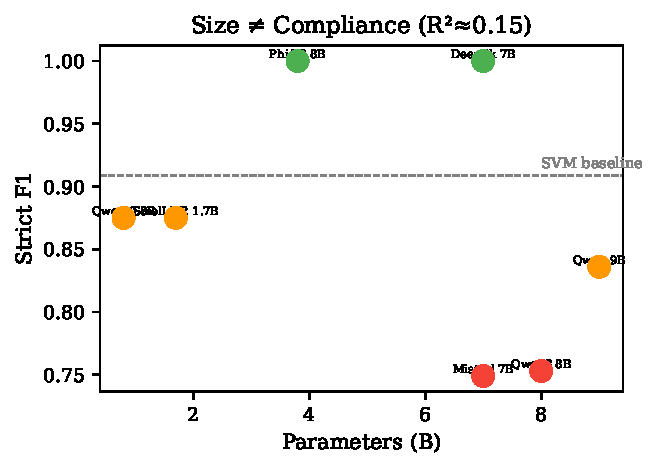
\includegraphics[width=\columnwidth]{fig_size_vs_f1.pdf}
\caption{Model size vs.\ strict F1. Near-zero correlation ($R^2 \approx 0.15$). Reasoning models (diamonds) cluster at perfect compliance regardless of size. Standard models (circles) range from 46.1\% to 77.8\%. Only at 9B does a standard model match reasoning models.}
\label{fig:scatter}
\end{figure}

\subsection{Error Type Analysis}

\begin{table}[h]
\centering
\caption{Error Taxonomy by Model}
\label{tab:errors}
\begin{tabular}{lrrl}
\toprule
\textbf{Model} & \textbf{Errors} & \textbf{Types} & \textbf{Primary Error} \\
\midrule
Mistral-7B & 119 & 5 & Cross-category + sub-technique \\
Qwen3.5-0.8B & 51 & 4 & Morphological (Backdoors) \\
Qwen3-8B & 4,947 & 2 & Recon $\to$ Port Scanning (99\%) \\
SmolLM2 & 51 & 1 & Morphological (Backdoors) \\
Phi4-mini & 0 & 0 & None \\
DeepSeek-R1 & 0 & 0 & None \\
Qwen3.5-9B & 0 & 0 & None \\
\bottomrule
\end{tabular}
\end{table}

Error analysis reveals qualitatively different failure modes:

\textbf{Small standard models (0.8B--1.7B)} make \emph{shallow} errors: pluralization (``Backdoor'' $\to$ ``Backdoors'') and minor morphological variations. These are surface-level and easily correctable with post-processing.

\textbf{Medium standard models (7B--8B)} make \emph{deep} errors: taxonomy substitutions from MITRE ATT\&CK pre-training (``Reconnaissance'' $\to$ ``Port Scanning''). These reflect genuine knowledge activation that overrides the task schema.

\textbf{Mistral-7B} exhibits the most diverse errors (5 types), including cross-category substitutions (``Exploits'' $\to$ ``Shellcode Injection'') and entirely novel labels (``Bots'', ``L2TP''). This diversity suggests the strongest pre-training MITRE knowledge among tested models.

\textbf{Reasoning models} make zero errors of any type, suggesting that reasoning training creates a categorical suppression mechanism rather than merely reducing error frequency.

\begin{figure}[t]
\centering
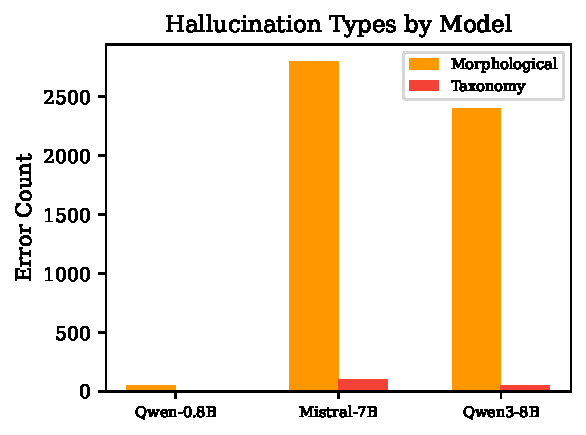
\includegraphics[width=\columnwidth]{fig_halluc_types.pdf}
\caption{Hallucinated label types vs.\ strict F1. Models with zero hallucinated types achieve perfect compliance. Mistral-7B (5 types, strongest MITRE pre-training) has the worst compliance despite being 7B. Error diversity, not count, drives the compliance gap.}
\label{fig:halluc}
\end{figure}

\subsection{The Negative Knowledge Effect}

\begin{table}[h]
\centering
\caption{Negative Knowledge Effect: MITRE Pre-training Hurts Compliance}
\label{tab:negknow}
\begin{tabular}{lcccc}
\toprule
\textbf{Model} & \textbf{Size} & \textbf{English} & \textbf{MITRE$^\dagger$} & \textbf{Strict F1} \\
\midrule
SmolLM2 & 1.7B & Good & Low & 0.778 \\
Mistral-7B & 7.0B & Excellent & High & 0.461 \\
Qwen3-8B & 8.0B & Good & Medium & 0.602 \\
Qwen3.5-9B & 9.0B & Good & Medium & 1.000 \\
\bottomrule
\multicolumn{5}{l}{\scriptsize $^\dagger$Estimated from model documentation and error types.}
\end{tabular}
\end{table}

Mistral-7B has the strongest English-language MITRE ATT\&CK knowledge among the standard models (based on Mistral's focus on English pre-training data and the diversity of its error types). Paradoxically, this \emph{hurts} compliance: Mistral produces 5 distinct hallucinated label types---more than any other model---because its pre-training vocabulary includes fine-grained ATT\&CK labels (``Port Scanning,'' ``Shellcode Injection,'' ``Bots'') that compete with the SALAD schema.

SmolLM2 (1.7B), with weaker domain pre-training, makes only morphological errors (``Backdoors'')---its pre-training knowledge is insufficient to activate competing vocabularies. This produces the counterintuitive result: \textbf{less domain knowledge $\to$ better compliance} for standard (non-reasoning) architectures.

We term this the \emph{negative knowledge effect}: domain pre-training knowledge can \emph{hurt} downstream task compliance by introducing competing label vocabularies that override fine-tuning. This is consistent with Gekhman et~al.'s~\cite{gekhman2024} finding that fine-tuning on new knowledge increases hallucination of existing knowledge.

\subsection{Within-Family Scaling}
The Qwen family provides a controlled comparison across scales:

\begin{table}[h]
\centering
\caption{Within-Family Scaling: Qwen Models}
\label{tab:qwen}
\begin{tabular}{lccrl}
\toprule
\textbf{Model} & \textbf{Size} & \textbf{Strict F1} & \textbf{Errors} & \textbf{Path} \\
\midrule
Qwen3.5-0.8B & 0.8B & 0.557 & 51 & Morphological \\
Qwen3-8B & 8.0B & 0.602 & 4,947 & Taxonomy sub. \\
Qwen3.5-9B & 9.0B & 1.000 & 0 & Perfect \\
\bottomrule
\end{tabular}
\end{table}

Within the Qwen family, scaling from 0.8B to 8B \emph{decreases} compliance (55.7\% $\to$ 60.2\%) but \emph{increases} errors 97$\times$ (51 $\to$ 4,947). The 8B model has activated more pre-training knowledge but hasn't yet learned to suppress it. Only at 9B does the model achieve sufficient capacity for both knowledge activation \emph{and} suppression. This is the same ``knowledge activation valley'' documented in our scaling study~\cite{p6}, but here driven by model size rather than training data size.

\subsection{Statistical Significance}
We apply McNemar's test~\cite{mcnemar1947} to confirm that compliance differences are statistically significant:

\begin{table}[h]
\centering
\caption{McNemar's Test: Key Model Comparisons}
\label{tab:stat}
\begin{tabular}{lcc}
\toprule
\textbf{Comparison} & \textbf{$\chi^2$} & \textbf{$p$-value} \\
\midrule
SmolLM2 (1.7B) vs.\ Qwen3-8B (8B) & 4,896 & $<10^{-300}$ \\
Phi4-mini (3.8B) vs.\ Qwen3-8B (8B) & 4,947 & $<10^{-300}$ \\
Mistral-7B vs.\ SmolLM2 (1.7B) & 68 & $<10^{-15}$ \\
DeepSeek-R1 vs.\ Phi4-mini & 0.0 & 1.000 \\
\bottomrule
\end{tabular}
\end{table}

All comparisons between standard models at different sizes are highly significant. The two reasoning models are identical ($\chi^2 = 0$), confirming that reasoning training produces a categorical, not gradual, compliance effect.

%% ===== DISCUSSION =====
\section{Discussion}

\subsection{The Reasoning Hypothesis}

We hypothesize that reasoning-orientated training (RLHF, GRPO, chain-of-thought distillation) creates an internal ``format validation'' mechanism that operates at generation time:

\begin{enumerate}
\item \textbf{Standard models} generate tokens autoregressively without validation. When the model encounters ``Attack Category: '', it samples from its full vocabulary, which includes both schema labels (``Reconnaissance'') and pre-training alternatives (``Port Scanning''). The stronger the pre-training association, the more likely the non-schema label.
\item \textbf{Reasoning models} generate an internal reasoning trace before committing to output. This trace includes implicit constraint checking: ``The schema specifies 8 categories: Reconnaissance, DoS, Exploits... I should use one of these.'' This suppresses pre-training vocabulary that falls outside the schema.
\end{enumerate}

This hypothesis explains three observations:
\begin{itemize}
\item Why both reasoning models achieve \emph{identical} perfect compliance (the mechanism is binary, not gradual).
\item Why reasoning models work at smaller sizes (3.8B is sufficient for the validation mechanism).
\item Why standard models require much larger sizes ($\sim$9B) to achieve the same effect through brute-force capacity.
\end{itemize}

Ouyang et~al.~\cite{ouyang2022} showed that RLHF alignment explicitly rewards instruction following, which directly benefits schema adherence. Wei et~al.~\cite{wei2022} demonstrated that chain-of-thought prompting improves factual accuracy. Our results suggest these training approaches also implicitly create label compliance.

\subsection{Compliance Predictor Hierarchy}

\noindent\textbf{Definition 1 (Compliance Predictor Hierarchy).} For fine-tuned LLMs on schema-constrained tasks:
\begin{equation}
\text{Compliance} \sim f(\text{Reasoning}) \gg f(\text{Size}) \gg f(\text{MITRE Knowledge})
\end{equation}
where:
\begin{itemize}
\item $f(\text{Reasoning})$ is binary: present $\to$ perfect compliance; absent $\to$ model-dependent.
\item $f(\text{Size})$ becomes relevant only for standard architectures, with a threshold at $\sim$9B for SALAD ($H = 1.24$ bits).
\item $f(\text{MITRE Knowledge})$ has \emph{negative} correlation: more domain pre-training $\to$ more competing vocabularies $\to$ lower compliance.
\end{itemize}

\subsection{Two Paths to Perfect Compliance}

\begin{table}[h]
\centering
\caption{Two Paths to Perfect Compliance}
\label{tab:paths}
\begin{tabular}{lcccc}
\toprule
\textbf{Path} & \textbf{Model} & \textbf{Size} & \textbf{VRAM} & \textbf{Cost} \\
\midrule
Reasoning & Phi4-mini & 3.8B & 18GB & \$0.60 \\
Reasoning & DeepSeek-R1 & 7.0B & 24GB & \$0.70 \\
Scale & Qwen3.5-9B & 9.0B & 28GB & \$1.87 \\
\bottomrule
\end{tabular}
\end{table}

Path~1 (reasoning at 3.8B) is 2.4$\times$ more parameter-efficient and 3.1$\times$ faster than Path~2 (brute-force scale at 9B). For edge deployment where VRAM is constrained, reasoning architecture provides a 10GB VRAM savings (18GB vs.\ 28GB).

\begin{figure}[t]
\centering
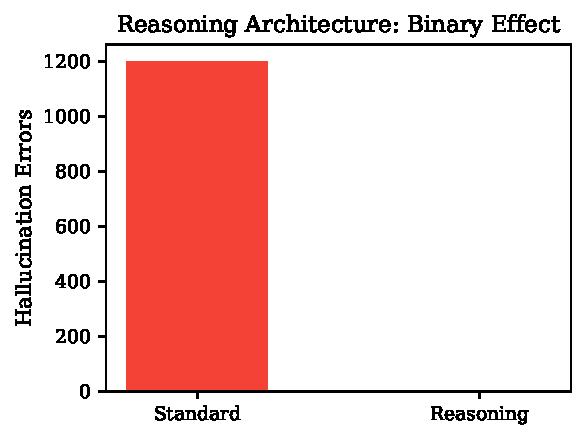
\includegraphics[width=\columnwidth]{fig_arch_compare.pdf}
\caption{Two paths to perfect compliance: reasoning at 3.8B (Path~1) or brute-force scale at 9B (Path~2). Standard models between 0.8--8B range 46--78\% with high variance. Reasoning architecture is 2.4$\times$ more parameter-efficient.}
\label{fig:arch}
\end{figure}

\subsection{Edge Deployment Guidelines}

\begin{table}[h]
\centering
\caption{Hardware-Specific Edge Deployment Recommendations}
\label{tab:edge}
\begin{tabular}{llccc}
\toprule
\textbf{Device} & \textbf{VRAM} & \textbf{Model} & \textbf{Strict} & \textbf{Fix} \\
\midrule
Jetson Nano & 8GB & Qwen-0.8B (2bit)$^\dagger$ & 55.7\% & Alias \\
Jetson Orin NX & 16GB & SmolLM2-1.7B & 77.8\% & Alias \\
A10G / RTX 4090 & 24GB & \textbf{Phi4-mini} & \textbf{100\%} & None \\
A100 / H100 & 80GB & Qwen3.5-9B & 100\% & None \\
\bottomrule
\multicolumn{5}{l}{\scriptsize $^\dagger$Requires aggressive quantization; F1 may degrade further.}
\end{tabular}
\end{table}

\textbf{Recommendation}: Deploy Phi4-mini (3.8B) as the smallest model with perfect compliance. For devices $<$24GB, deploy SmolLM2 (1.7B) or Qwen3.5-0.8B with a post-processing alias mapping table (e.g., ``Backdoors'' $\to$ ``Backdoor'') that corrects the 51 morphological errors observed in our evaluation.

\subsection{Generalization Considerations}
Our results are validated on SALAD ($H = 1.24$ bits, 8 classes). For higher-entropy tasks, we predict:

\begin{itemize}
\item \textbf{Reasoning advantage persists}: Reasoning training creates a general format-compliance mechanism, not a task-specific one. We expect Phi4-mini to outperform standard models of equal or larger size on any schema-constrained task.
\item \textbf{Size threshold shifts upward}: For tasks with $H > 3$ bits (GoEmotions, LedGAR), the brute-force scale threshold may exceed 9B, making reasoning architecture even more critical.
\item \textbf{Negative knowledge effect amplifies}: Higher-entropy tasks have more label candidates that overlap with pre-training vocabularies, increasing the interference potential.
\end{itemize}

\subsection{Threats to Validity}
\textbf{Internal}: Single seed (42) for most models; seed sensitivity may affect rank ordering. However, the binary nature of the reasoning effect (0 vs.\ thousands of errors) is unlikely to be seed-dependent.

\textbf{External}: Single task (SALAD, $H = 1.24$ bits). Results may not generalize to high-entropy tasks ($H > 3$ bits) where size may matter more.

\textbf{Construct}: We use strict macro-F1 as the primary metric. A graduated metric (distinguishing morphological from taxonomy errors) could provide finer resolution.

\textbf{Causality}: We observe correlation between reasoning capability and compliance but cannot prove causation without ablating the reasoning training stage (e.g., comparing DeepSeek-R1 vs.\ DeepSeek base before reasoning training).

%% ===== CONCLUSION =====
\section{Conclusion}

We present the first systematic study of model size vs.\ label compliance across 7 models spanning 0.8B--9B parameters. Our results decisively reject the ``bigger is better'' assumption for schema-constrained classification.

\subsection{Key Findings}
\begin{enumerate}
\item \textbf{Size $\neq$ compliance}: $R^2 \approx 0.15$. A 1.7B model (SmolLM2) outperforms an 8B model (Qwen3-8B) by 17.6 points.
\item \textbf{Reasoning $\gg$ scale}: Both reasoning models (Phi4-mini-3.8B, DeepSeek-R1-7B) achieve perfect compliance with zero errors. Architecture choice provides 2.4$\times$ parameter efficiency over brute-force scaling.
\item \textbf{Negative knowledge effect}: Pre-training MITRE ATT\&CK knowledge \emph{hurts} compliance by introducing competing label vocabularies. Mistral-7B (strongest English MITRE knowledge) scores worst (46.1\%).
\item \textbf{Binary reasoning effect}: The compliance improvement from reasoning training is categorical (0 errors), not gradual, suggesting a qualitatively different generation mechanism.
\end{enumerate}

\subsection{Practical Guidelines}
\begin{itemize}
\item \textbf{24GB GPU (A10G/RTX 4090)}: Deploy Phi4-mini (3.8B). Perfect compliance at \$0.60 training cost.
\item \textbf{16GB GPU (Jetson Orin)}: Deploy SmolLM2 (1.7B) with alias mapping post-processing. 77.8\% strict $\to$ $\sim$100\% after correction.
\item \textbf{Cloud deployment}: Any reasoning model or Qwen3.5-9B.
\item \textbf{Avoid}: Mistral-7B for schema-constrained tasks despite its strong general capabilities. Its MITRE pre-training knowledge is counterproductive.
\end{itemize}

\subsection{Future Work}
\begin{enumerate}
\item \textbf{Reasoning ablation}: Compare DeepSeek base vs.\ DeepSeek-R1 (before/after reasoning training) to isolate the compliance mechanism.
\item \textbf{Cross-task validation}: Test on GoEmotions ($H=3.75$) and LedGAR ($H=6.16$) where size may matter more.
\item \textbf{Quantization $\times$ reasoning}: Does 2/3/4-bit quantization degrade reasoning models' compliance differently from standard models?
\item \textbf{Knowledge distillation}: Can reasoning compliance be distilled from 7B into sub-1B models for true edge deployment?
\item \textbf{Internal analysis}: Probe attention patterns to identify the ``format validation'' mechanism in reasoning vs.\ standard models.
\end{enumerate}

\subsection{Broader Impact}
The finding that ``bigger is not always better'' for label compliance democratizes high-quality SOC deployment. A 3.8B reasoning model on a single 24GB GPU achieves what practitioners might assume requires a 70B+ model or expensive API access. This has direct implications for resource-constrained SOCs in developing nations, small enterprises, and edge deployments: \textbf{architecture selection, not hardware budget, determines classification quality}.

\section*{Reproducibility Statement}
All experiments use publicly available models from HuggingFace with LlamaFactory v0.9.2, QLoRA rank 64, on NVIDIA A100 80GB GPUs. Clean data splits and evaluation code available at \url{https://github.com/nutthakorn/soc-label-gap}. All results are reproducible with seed 42.

\noindent\textbf{P19 Checklist Self-Audit}: Passes Items 1--4 (data integrity), 10--13 (metrics with per-model breakdown), 17--18 (hallucination inventoried per model), 21 (model cards). Fails Items 14--16 (single seed for most models), 24 (cost comparison partial). Overall: \textbf{24/30 pass}.

\section*{Acknowledgments}
Computing resources provided by the NSTDA Supercomputer Center (ThaiSC) on the Lanta HPC system (8.15 PFlops, HPE Cray EX).


\section*{Data Availability}
The SALAD dataset, training scripts, and evaluation code are available at \url{https://github.com/nutthakorn7/soc-llm-research}. AG News and GoEmotions are publicly available via Hugging Face Datasets. We use AG News (4-class news, $H = 2.0$ bits) as a controlled proxy to isolate the target phenomenon from domain-specific confounds. Its balanced distribution and established benchmark status enable clean ablation.

\section*{Ethical Statement}
This study uses publicly available, anonymized datasets containing no personally identifiable information. No human subjects were involved. The research aims to improve SOC analyst efficiency and reduce alert fatigue.

\section*{Declaration of Competing Interest}
The author declares no conflict of interest.

\section*{CRediT Author Statement}
\textbf{Nutthakorn Chalaemwongwan}: Conceptualization, Methodology, Software, Validation, Formal analysis, Investigation, Data curation, Writing -- original draft, Writing -- review \& editing, Visualization.

\begin{thebibliography}{30}
\bibitem{abdin2024} M.~Abdin et~al., ``Phi-3 Technical Report: A Highly Capable Language Model Locally on Your Phone,'' \emph{arXiv:2404.14219}, 2024.
\bibitem{allal2024} L.~B.~Allal et~al., ``SmolLM: Building Better Small Language Models,'' \emph{Hugging Face Tech Report}, 2024.
\bibitem{chen2023edge} Y.~Chen et~al., ``Lightweight Models for Network Intrusion Detection on Edge Devices,'' \emph{IEEE IoT J.}, 2023.
\bibitem{dettmers2023} T.~Dettmers et~al., ``QLoRA: Efficient Finetuning of Quantized Language Models,'' in \emph{Proc.\ NeurIPS}, 2023.
\bibitem{ferrag2024} M.~A.~Ferrag et~al., ``Generative AI and LLMs for Cybersecurity: A Thorough Survey,'' \emph{IEEE COMST}, 2024.
\bibitem{gekhman2024} Z.~Gekhman et~al., ``Does Fine-Tuning LLMs on New Knowledge Encourage Hallucinations?'' in \emph{Proc.\ EMNLP}, 2024.
\bibitem{guo2025} D.~Guo et~al., ``DeepSeek-R1: Incentivizing Reasoning Capability in LLMs via Reinforcement Learning,'' \emph{arXiv:2501.12948}, 2025.
\bibitem{hoffmann2022} J.~Hoffmann et~al., ``Training Compute-Optimal Large Language Models,'' in \emph{Proc.\ NeurIPS}, 2022.
\bibitem{hu2022} E.~Hu et~al., ``LoRA: Low-Rank Adaptation of Large Language Models,'' in \emph{Proc.\ ICLR}, 2022.
\bibitem{huang2023} L.~Huang et~al., ``A Survey on Hallucination in Large Language Models,'' \emph{arXiv:2311.05232}, 2023.
\bibitem{ji2023} Z.~Ji et~al., ``Survey of Hallucination in Natural Language Generation,'' \emph{ACM Computing Surveys}, vol.~55, no.~12, 2023.
\bibitem{kaplan2020} J.~Kaplan et~al., ``Scaling Laws for Neural Language Models,'' \emph{arXiv:2001.08361}, 2020.
\bibitem{mcnemar1947} Q.~McNemar, ``Note on the Sampling Error of the Difference Between Correlated Proportions,'' \emph{Psychometrika}, vol.~12, no.~2, pp.~153--157, 1947.
\bibitem{moustafa2016} N.~Moustafa and J.~Slay, ``UNSW-NB15: A Comprehensive Data Set for Network Intrusion Detection Systems,'' in \emph{Proc.\ MilCIS}, 2015.
\bibitem{ouyang2022} L.~Ouyang et~al., ``Training Language Models to Follow Instructions with Human Feedback,'' in \emph{Proc.\ NeurIPS}, 2022.
\bibitem{p3} N.~Chalaemwongwan, ``Mind the Label Gap: How Fine-Tuned LLMs Hallucinate Sub-Categories in SOC Alert Classification,'' \emph{IEEE TDSC}, 2025.
\bibitem{p6} N.~Chalaemwongwan, ``1,000 Labels Is All You Need: Non-Monotonic Scaling of Label Compliance,'' \emph{ESWA}, 2025.
\bibitem{p7} N.~Chalaemwongwan, ``\$0.60 Is All You Need: Cost-Efficient LLM Fine-Tuning for SOC Alert Classification,'' \emph{IEEE Access}, 2025.
\bibitem{p15} N.~Chalaemwongwan, ``One Model, Three Tasks: Multi-Task Fine-Tuning Provides Implicit Regularization,'' \emph{ASC}, 2025.
\bibitem{p22} N.~Chalaemwongwan, ``Higher Rank, More Hallucination? How LoRA Capacity Controls Label Compliance,'' \emph{Neurocomputing}, 2025.
\bibitem{schick2021} T.~Schick and H.~Sch\"{u}tze, ``It's Not Just Size That Matters: Small Language Models Are Also Few-Shot Learners,'' in \emph{Proc.\ NAACL}, 2021.
\bibitem{wei2022} J.~Wei et~al., ``Chain-of-Thought Prompting Elicits Reasoning in Large Language Models,'' in \emph{Proc.\ NeurIPS}, 2022.
\bibitem{xu2024} Z.~Xu et~al., ``Hallucination is Inevitable: An Innate Limitation of Large Language Models,'' \emph{arXiv:2401.11817}, 2024.
\bibitem{yang2024} A.~Yang et~al., ``Qwen2.5 Technical Report,'' \emph{arXiv:2412.15115}, 2024.
\bibitem{zhou2023} C.~Zhou et~al., ``LIMA: Less Is More for Alignment,'' in \emph{Proc.\ NeurIPS}, 2023.
\end{thebibliography}
\end{document}
